% !TEX root = ../Vorlage_DA.tex
%	########################################################
% 					Autoren
%	########################################################


%	--------------------------------------------------------
% 	Überschrift, Inhaltsverzeichnis
%	--------------------------------------------------------
\chapter*{Autoren}
\addcontentsline{toc}{chapter}{Authoren}

%	--------------------------------------------------------
% 	Autor 1
%	--------------------------------------------------------
\htlParagraph{Frieda Fröhlich}

\renewcommand{\arraystretch}{1.2}
\begin{tabularx}{1\textwidth}{@{} l X l @{}}

\emph{Geburtstag, Geburtsort:} & 01.01.1970, Braunau am Inn & 
\multirow{5}{2.5cm}{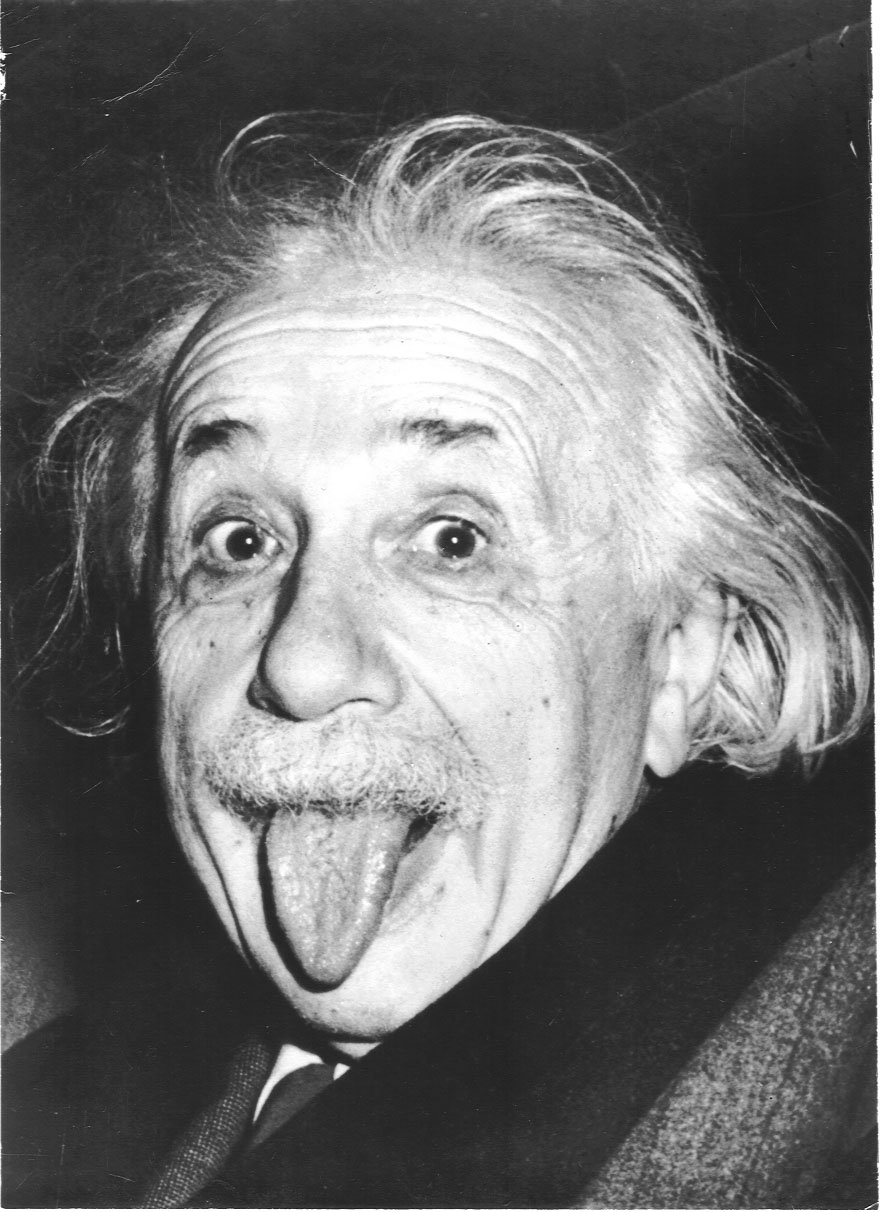
\includegraphics[width=2.5cm]{./media/images/einstein.jpg}
} 
\\
\emph{Schulbildung:} & Volksschule \newline Hauptschule \newline HTL & \\
\emph{Praktika:} & Firmenname, Zeit, Tätigkeit & \\
\emph{Anschrift:} & Strasse Nummer\newline PLZ, Ort\newline Österreich & \\
\emph{E-Mail:} & frieda@froehlich.com & \\

\end{tabularx}
\\\\
%	--------------------------------------------------------
% 	Autor 1
%	--------------------------------------------------------
\htlParagraph{Max Mustermann}

\begin{tabularx}{1\textwidth}{@{} l X l @{}}
\emph{Geburtstag, Geburtsort:} & 01.01.1970, Braunau am Inn & 
\multirow{5}{2.5cm}{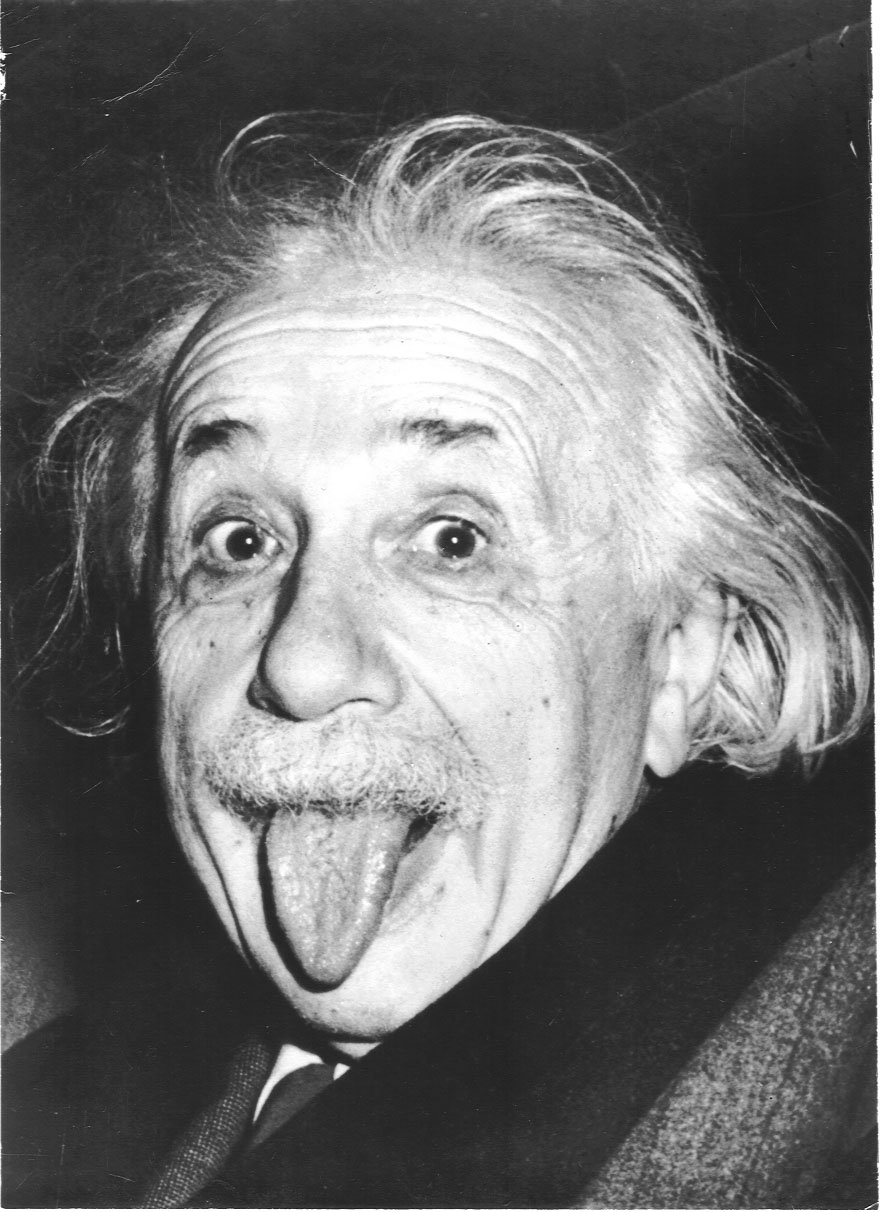
\includegraphics[width=2.5cm]{./media/images/einstein.jpg}
} 
\\
\emph{Schulbildung:} & Volksschule \newline Hauptschule \newline HTL & \\
\emph{Praktika:} & Firmenname, Zeit, Tätigkeit & \\
\emph{Anschrift:} & Strasse Nummer\newline PLZ, Ort\newline Österreich & \\
\emph{E-Mail:} & max@mustermann.com & \\

\end{tabularx}
